\section{Colonia de Hormigas}
\label{sec:intro}

En nuestro mundo natural, las hormigas (inicialmente) vagan de manera aleatoria, al azar, y una vez encontrada comida regresan a su colonia dejando un rastro de feromonas. Si otras hormigas encuentran dicho rastro, es probable que estas no sigan caminando aleatoriamente, puede que estas sigan el rastro de feromonas, regresando y reforzándolo si estas encuentran comida finalmente.


Es una methaeuristica de la familia de SI (Swarm intelligence) basada en el comportamiento en grupo de las hormigas para encontrar el mejor camino a un recurso.

En un principio todas las hormigas de mueven de manera aleatoria buscando un camino al recurso deseado (una solucion). Una vez encontrado el recurso la hormiga vuelve dejando un rastro de feromonas, que puede depender de que tan buena sea la solucion. Utilizando este rastro se comparte información entre las hormigas.

Cuando una hormiga comienza su trabajo, es influenciada por la feromona depositada por las hormigas anteriores, aumentando asi las posibilidades de encontrar una solucion mejor a la ya encontrada.

\begin{figure}[h]
	\centering
	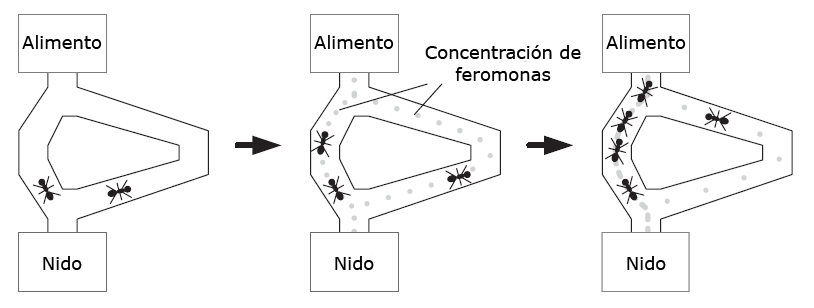
\includegraphics[scale=0.4]{./img/colonia_ejemplo.png}
	\caption{Colonia de hormigas}
	\label{img:ants}
\end{figure}

Esta feromona además tiene un factor de evaporación, esto produce que los caminos pierdan
su fuerza de atracción, cuanto más largo sea el camino, más tiempo demorará una hormiga
en recorrerlo, más se evaporará la feromona y por ende serán menos frecuentado. Por su parte
los caminos más cortos (o más óptimos) tendrán mayor cantidad de feromonas, por ende, mayor
probabilidad de ser frecuentados. Además, nos da la ventaja de evitar convergencias a optiomos locales.
Figura \ref{img:ants}.

El algritmo general de Colonia de Hormigas consiste en dos loops principales. 
Por cada ciclo principal, todas las hormigas buscan una solucion que luego es 
comparada con la mejor solucion al momento, actualizando la feromona corresponientemente. Tambien,
luego de cada ciclo principal, se implementa  el mecanismo de evaporacion. 

\clearpage

\subsection{Colonia de hormigas para Sudoku}

Decidimos implementar la metaheristicas de Colonia de Hormigas siguiendo las 
ideas principales del paper de Krzysztof Schif \cite{ant_colony}, tomando 
algunas decisiónes que no estaban explicitas en el mismo.

El paper plantea la utilizacion de una matriz tridimencional $T$ para guardar la 
feromona. Asi, por casa posicion en la grilla (fila, columna) y por cada digito (del 1 al 9) 
se ira almacenando la feromona de acuerdo a si en determinada fila y columna 
determinado digito es parte o no de la solucion. Al principo del algoritmo se 
inicializa la matriz con un valor inicial.

Como todo algoritmo de Colonia de Hormigas, este se compone de 2 ciclos 
principales, uno para repetir el trabajo en conjunto de las hormigas y uno en el 
cual cada hormiga realiza su trabajo. 

El trabajo de cada hormiga es buscar una solucion, utilizando la informacion 
depositada en la matriz $T$ por las iteraciones anteriores. En un principio las 
hormigas intentan llenar todos los lugares posibles del $Sudoku$. Esto pasa 
debido a que en un determinado momento en el tablero puede haber posiciones a 
las cuales unicamente se les puede asignar un único valor. Para esto vamos 
guardando en una matriz $digits$ para cada posicion en el tablero cuantos digitos estan disponibles.  

\begin{figure}[h]
	\centering
	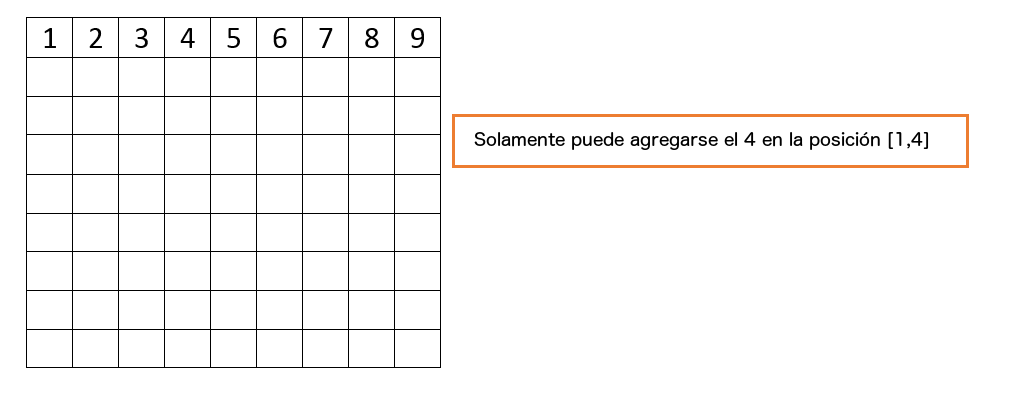
\includegraphics[scale=0.4]{./img/soloundigitoa.png}
	\caption{Ant colony}
	\label{img:soloundigito}
\end{figure}

Tambien puede ocurrir que en en una posicion de una subgrilla solo se pueda 
colocar un digito. Para esto nos vamos guardando en otra matriz $places$ para 
cada posicion y digito, la cantidad de opciones dentro de la submatriz.

\begin{figure}[h]
	\centering
	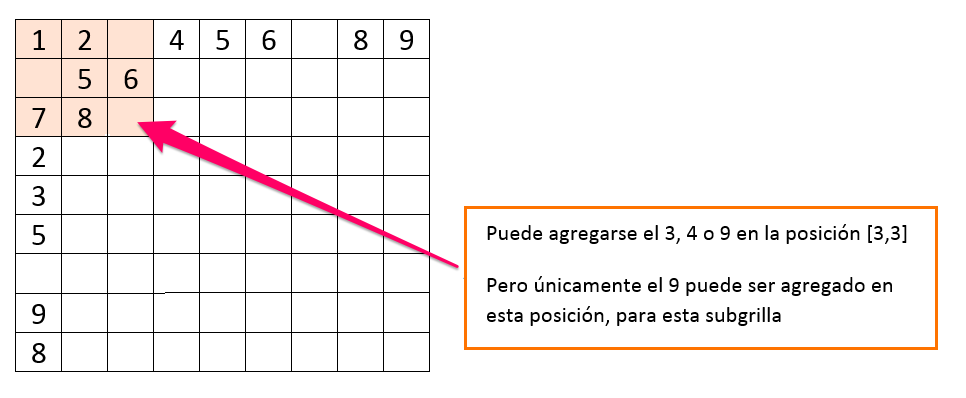
\includegraphics[scale=0.4]{./img/undigitosolo.png}
	\caption{Ant colony}
	\label{img:soloundigito}
\end{figure}

Una vez que la hormiga coloco todos los digitos que puedo, la hormiga debe 
decidir cual es el siguiente digito a colocar en la grilla. Para esto calcula 
para cada posicion y digito la probabilidad a ser agregada, utilizando la 
feromona y la composicion de la solucion hasta el momento. 

Una vez calculadas estas probabilidades, lo que se hace es ordenar las 
posibilidades por esta probabilidad y quedarse con un elemento al azar entre un 
porcentage de las que mas probabilidades tiene. Aca es donde entra la parte 
probabilistica del algoritmo, por lo cual cada hormiga llega a una potencial 
solucion distinta.


\begin{Verbatim}[samepage=true]
def next_to_add
  probabilidades = calcularProbabilidades
  ordernado = ordernarPorProbabilidad(probabilidades)
  losMasProbables = losElementosConMasProbabilidad(ordenado)
  losMasProbables.sample
end
\end{Verbatim}


Una vez agregado este digito, se vuelve a repetir el ciclo de agregar los 
digitos que solo van en un lugar y volviendo luego a elegir el siguiente utilizando el metodo recien descripto.
Este ciclo de la hormiga termina cuando:

\begin{itemize}
	\item Ya no tiene posibles posiciones en las cuales agregar un dígito.
	\item Cuando encuentra al menos una posición en la cual no agregar un dígito.
\end{itemize}

Una vez finalizado el trabajo de la hormiga, se compara su solucion con la mejor 
hasta el momento actualizandola si esto en necesario.

Cuando el trabajo de todas las hormigas finaliza, se procede a actualizar la feromona. 
Por un lado se aplica la evaporacion correspondiente y por el otro se actualiza 
la fermona para aquellas posiciones y digitos que pertencen a la mejor solucion obtenida por las hormigas en el ciclo.
Por otro lado se compara con la solucion global para actualizarla también si es 
mejor que la misma.

El pseudo-código a grandes rasgos queda de la siguiente manera:

\begin{Verbatim}[samepage=true]
forEach ciclo {
  forEach hormiga {
    solucionParcialDeHormiga = realizarTrabajoDeHormiga
    
    if (solucionParcialDeHormiga es mejor que solucionParcial ) {
      solucionParcial = solucionParcialDeHormiga
    }
  }
  
  aplicarEvaporacion()
  actualizarFeromona(solucionParcial)
  
  if (solucionParcial es mejor que solucionFinal ) {
    solucionFinal = solucionParcial
  }
}
\end{Verbatim}









